\chapter*{Wstęp}
\label{cha:wstęp}

\section*{Wprowadzenie}
\label{sec:wprowadzenie}

Cyfrowe przetwarzanie sygnałów, \ac{dsp} jest dziedziną inżynierii zajmującą się metodami przetwarzania oraz analizy sygnałów cyfrowych. Źródłem sygnałów cyfrowych mogą być między innymi przetworniki analogowo-cyfrowe (A/C) oraz generatory sygnałów. Najpopularniejszymi przykładami sygnałów analogowych konwertowanych do domeny cyfrowej są sygnały odbierane ze źródeł audio oraz sygnały wideo.

Algorytmy przetwarzania sygnałów znajdują szerokie zastosowanie w wielu dziedzinach techniki, takich jak telekomunikacja (np. w systemach komunikacji mobilnej), obróbka dźwięku (np. w equalizerach) oraz bezpieczeństwo danych (np. szyfrowanie). Przykładowe algorytmy wykorzystywane we wspomnianych zastosowaniach obejmują transformacje takie jak \ac{fft}, umożliwiające analizę sygnałów w dziedzinie częstotliwości; filtry \ac{dsp}, zarówno liniowe, jak i nieliniowe, stosowane do eliminacji zakłóceń oraz optymalizacji jakości sygnału; oraz algorytmy szyfrowania, które zabezpieczają dane podczas transmisji.

Algorytmy przetwarzania sygnałów, mimo upływu lat (prace nad cyfrowym przetwarzaniem sygnałów rozpoczęły się w latach 50. XX wieku), pozostają tematem bardzo aktualnym, budzącym ciekawość wśród naukowców i inżynierów. Zastosowania \ac{dsp} rozwijają się dynamicznie, obejmując coraz nowsze obszary, co czyni tę dziedzinę niezbędną w rozwoju współczesnej technologii.

% \subsection*{Równoległe przetwarzanie danych}
% Algorytmy cyfrowego przetwarzania sygnałów (\ac{dsp}) stawiają wysokie wymagania wobec wydajności systemów obliczeniowych.
% Procesory, choć rozwijają się pod względem mocy obliczeniowej, napotykają ograniczenia wynikające z sekwencyjnego przetwarzania,
% co sprawia, że są mniej efektywne przy obliczeniach, które można prowadzić równolegle. W tym kontekście układy \ac{fpga} (Field-Programmable Gate Arrays) wyróżniają się
% możliwością równoległego przetwarzania danych, co pozwala na znaczne przyspieszenie złożonych operacji. Dzięki takiemu rozwiązaniu można przetwarzać wiele
% strumieni danych jednocześnie, co daje wyraźną przewagę nad procesorami, szczególnie w aplikacjach wymagających wysokiej przepustowości.

% \subsection*{Kontrola zegara i deterministyczne przetwarzanie}
% Kolejną zaletą układów \ac{fpga} jest możliwość precyzyjnego dostosowania częstotliwości zegara do wymagań projektowych. Dzięki wykorzystaniu języków opisu sprzętu,
% takich jak VHDL czy SystemVerilog, projektant ma pełną kontrolę nad wartościami sygałów w każdym takcie zegara, co umożliwia dokładne określenie, kiedy dane operacje mają się wykonywać.
% To daje pewność, że w takich aplikacjach jak filtr \ac{fir} dane będą przetwarzane i transmitowane w równych, określonych odstępach czasowych, co jest kluczowe. W odróżnieniu od procesorów,
% gdzie czas wykonywania kodu może być niedeterministyczny -- szczególnie w językach wysokiego poziomu, takich jak Python -- \ac{fpga} zapewniają
% pełną deterministyczność przetwarzania. Nawet w językach niskiego poziomu użytkownik nie zawsze ma pełną kontrolę nad czasem wykonywania kodu, ponieważ każda instrukcja wiąże się z pewnym narzutem czasowym.

\section*{Cel pracy}
\label{sec:cel_pracy}
% Część \ac{fpga} systemu jest odpowiedzialna za implementację
% algorytmów \ac{dsp}, zaś wbudowany procesor (HPS) pełni funkcję jednostki sterującej, uruchamiając serwer, który umożliwi użytkownikowi zdalną interakcję z systemem poprzez interfejs graficzny.

Celem niniejszej pracy była konstrukcja systemu do przetwarzania sygnałów cyfrowych w opraciu o system heterogeniczny, łączący w jednym układzie scalonym mikroprocesor \acsu{arm} oraz układ \ac{fpga}. Wykorzystanie takiego rozwiązania umożliwiło dystrybucję zadań pomiędzy aplikacje zarządzane przez system operacyjny Linux oraz układ cyfrowy zaimplementowany w FPGA.
% Kontrolę nad częścią systemu odpowiedzialną za \ac{dsp} według założeń miała pełnić aplikacja internetowa
% umożliwiająca użytkownikowi zdalną interakcję z układem.

Motywacją do realizacji projektu była potrzeba weryfikacji możliwości wykorzystania systemu heterogenicznego do przetwarzania sygnałów pochodzących z np. przetworników analogowo-cyfrowych (A/C) w czasie rzeczywistym. W wielu zastosowaniach przetwarzanie sygnałów wymaga możliwości dostosowania architektury systemu do specyficznych potrzeb aplikacji, czego mogą nie oferować inne rozwiązania oparte np. o mikrokontrolery lub procesory sygnałowe, \ac{dsp_proc}. Ponadto dzięki integracji  układu \ac{fpga} z \ac{hps}, użytkownik ma możliwość zdalnego zarządzania systemem oraz monitorowania przetwarzanych sygnałów, co zwiększa elastyczność i wygodę pracy. Umożliwia to szybkie dostosowywanie parametrów przetwarzania do konkretnych potrzeb, co jest istotne w wielu aplikacjach.

System ten ma na celu nie tylko zaprezentowanie w praktyce możliwości przetwarzania sygnałów, ale również stworzenie podstawy do dalszego rozwoju o kolejne funkcjonalności, takie jak implementacja nowych algorytmów \ac{dsp}, rozszerzenie interfejsu użytkownika, czy integracja z innymi systemami przetwarzania danych.
% Część \ac{fpga} systemu będzie odpowiedzialna za implementację algorytmów \ac{dsp}, w tym filtru \ac{fir} oraz modułu
% realizującego dyskretną transformatę Fouriera (DFT). System ten będzie wyposażony w dwie pamięci, pomiędzy którymi dane będą transmitowane, przetwarzane, a następnie zapisywane.
% Równocześnie wbudowany procesor będzie pełnił funkcję jednostki sterującej, uruchamiając serwer, który umożliwi użytkownikowi zdalną interakcję z systemem poprzez stronę internetową.
% Strona będzie umożliwiać wprowadzanie danych do FPGA, inicjowanie procesów przetwarzania oraz monitorowanie wyników. Taki podział zadań na układ \ac{fpga} i HPS umożliwia
% efektywną realizację algorytmów \ac{dsp}, zapewniając wysoką wydajność oraz intuicyjną obsługę przez użytkownika.

\section*{Zakres pracy}
\label{sec:zakresPracy}
Zakres pracy obejmował:
\begin{itemize}
    \item opracowanie systemu do transmisji danych zaimplementowanego w FPGA;
    \item implementację w systemie algorytmów \ac{dsp};
    \item przygotowanie środowiska uruchomieniowego w Yocto;
    \item stworzenie oprogramowania w języku Python;
    \item zaprojektowanie aplikacji internetowej.
\end{itemize}

W projekcie opracowano wydajny system transmisji danych oparty na \ac{fpga}, który umożliwia przesył i odczyt danych pomiędzy \ac{hps} a pamięciami w \ac{fpga}, z wykorzystaniem bezpośredniego dostępu do pamięci, \ac{dma}. Implementacja obejmowała algorytmy \ac{dsp}, w tym filtr \ac{fir} z możliwością dynamicznej zmiany współczynników, moduł \ac{fft} oraz algorytm enkrypcji danych. Stworzone oprogramowanie w języku Python, oparte na bibliotece unittest, umożliwiało testowanie i weryfikację funkcjonalności systemu, a także obsługę zadań po stronie FPGA. Ponadto zaprojektowano aplikację internetową, która umożliwia użytkownikowi zdalną interakcję z systemem.

% W ramach pracy powstała również strona internetowa, która pozwola użytkownikowi na przesył danych, komunikację z systemem oraz wizualizację wyników. Interfejs strony został zaprojektowany z myślą o intuicyjnej obsłudze,
% a także w sposób umożliwiający łatwą implementację kolejnych funkcjonalności w przyszłości.

\section*{Struktura pracy}
\label{sec:strukturaPracy}


% \begin{figure}[!htb]
%     \centerline{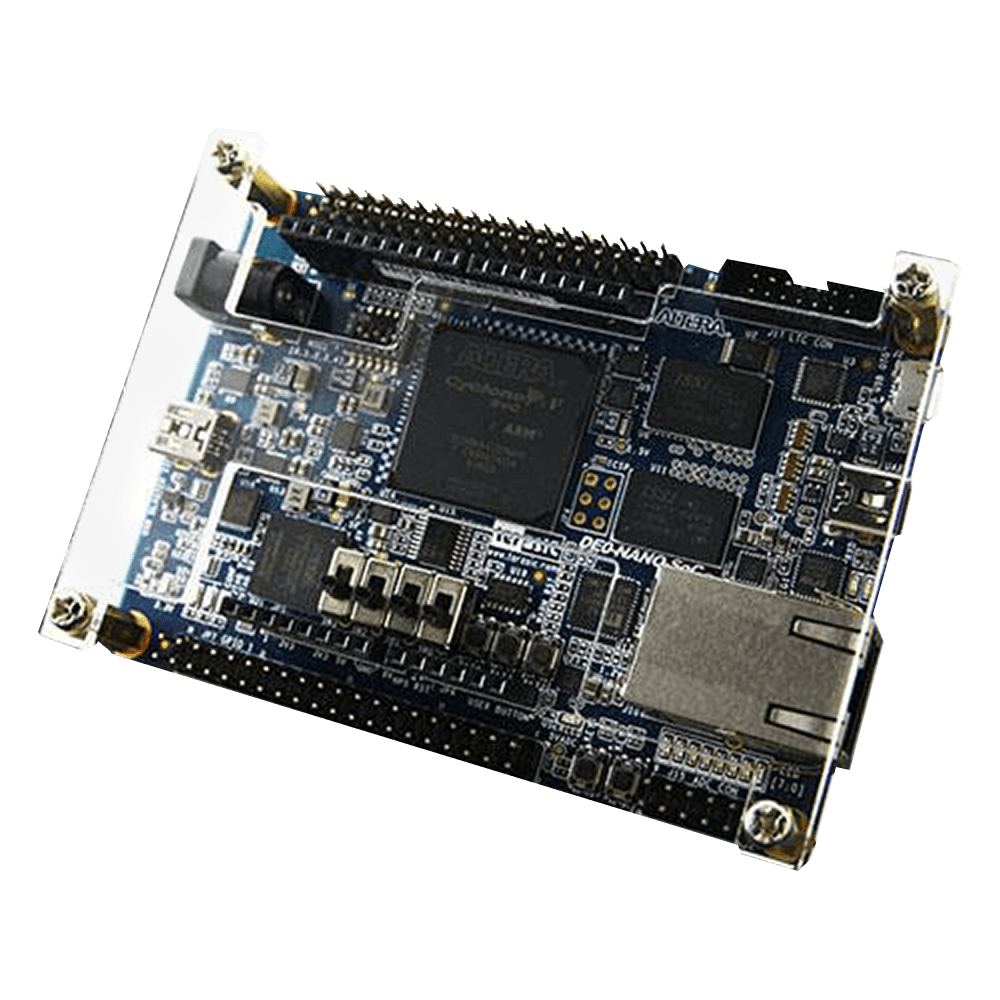
\includegraphics[scale=0.2]{de0-nano-soc.png}}
%     \caption{Układ DE0-Nano-SoC (Cyclone V)}
%     \label{fig:de0-nano-soc}
% \end{figure}



















